\documentclass[border=4pt]{standalone}
\usepackage{pgfplots}
\pgfplotsset{compat=1.18}

\begin{document}
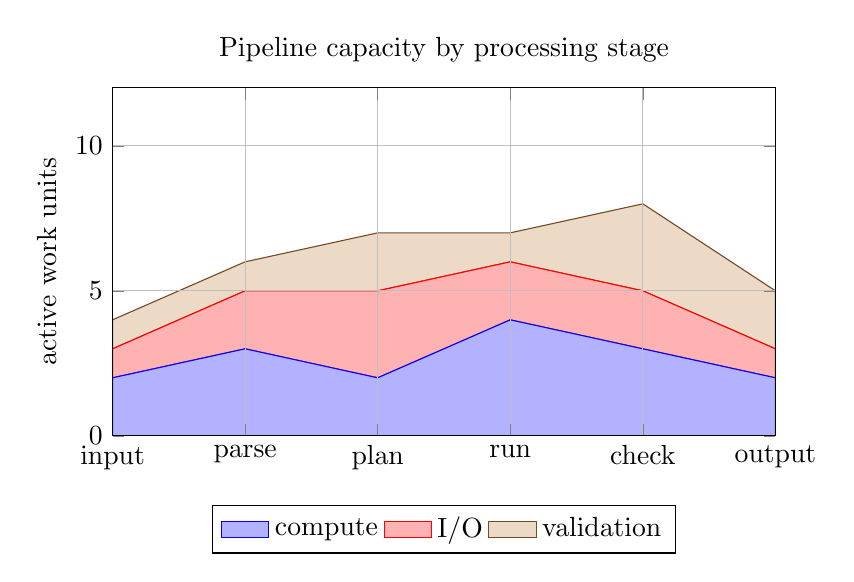
\begin{tikzpicture}
  \begin{axis}[
    stack plots=y,
    area style,
    width=10cm,
    height=6cm,
    xmin=0,
    xmax=5,
    ymin=0,
    ymax=12,
    enlargelimits=false,
    xtick={0,1,2,3,4,5},
    xticklabels={input,parse,plan,run,check,output},
    ylabel={active work units},
    title={Pipeline capacity by processing stage},
    grid=major,
    legend style={at={(0.5,-0.2)},anchor=north,legend columns=-1}
  ]
    \addplot coordinates {(0,2) (1,3) (2,2) (3,4) (4,3) (5,2)} \closedcycle;
    \addplot coordinates {(0,1) (1,2) (2,3) (3,2) (4,2) (5,1)} \closedcycle;
    \addplot coordinates {(0,1) (1,1) (2,2) (3,1) (4,3) (5,2)} \closedcycle;
    \legend{compute,I/O,validation}
  \end{axis}
\end{tikzpicture}
\end{document}
